\documentclass[10pt,twocolumn]{article}
\DeclareUnicodeCharacter{200A}{~}
% required packages for Oxy Comps style
\usepackage{oxycomps} % the main oxycomps style file
\usepackage{times} % use Times as the default font
\usepackage[style=numeric,sorting=nyt]{biblatex} % format the bibliography nicely
\usepackage{amsmath, amsthm, amssymb, amsfonts}
\usepackage{amsfonts} % provides many math symbols/fonts
\usepackage{listings} % provides the lstlisting environment
\usepackage{amssymb} % provides many math symbols/fonts
\usepackage{graphicx} % allows insertion of grpahics
\usepackage{hyperref} % creates links within the page and to URLs
\usepackage{url} % formats URLs properly
\usepackage{verbatim} % provides the comment environment
\usepackage{xpatch} % used to patch \textcite

\bibliography{references}
\DeclareNameAlias{default}{last-first}

\xpatchbibmacro{textcite}
  {\printnames{labelname}}
  {\printnames{labelname} (\printfield{year})}
  {}
  {}

\pdfinfo{
    /Title (Comps Proposal)
    /Author (Caleb Jordening)
}

\title{DRL in RL: Deep Reinforcement Learning in Rocket League}
\author{Caleb Jordening}
\affiliation{Occidental College}

\begin{document}

\maketitle

\section {Problem Context}

In the past few years, artificial intelligence (AI) has garnered quite the popularity from the media. From self-driving cars to smart-homes and virtual assistants, the future is quite hopeful for all of the technological innovations this field has to offer. Moreover, the sub-category of AI known as deep learning is using neural networks to help in the endeavor of reverse engineering the brain. These artificial neural networks can provide a model to let us understand more about how the biological brain works; and, hopefully, will allow us to produce general AI that possesses cognitive abilities greater than or equal to a human's. Currently, however, we are only able to produce narrow AI that can only perform a single task. 

\subsection{Search for General AI}
In the search for creating general AI, board games and video games provide a high-dimensional, goal-oriented environment in which learning algorithms can be implemented to achieve the goal of the game. Games provide a structure that allows for learning algorithms to be implemented so that the AI can become more adept to learning, which could then potentially generalise to real life applications — resulting in the emergence of general AI. The three most prominent methods for machine learning are: supervised learning, unsupervised learning, and reinforcement learning. Of these three, reinforcement learning is arguably the best suited for training an agent to play a game. Board and video games possess states, rewards, and actions. A person playing the game provides certain inputs that result in actions in the game. Actions are performed to reach a particular state of the game; which, in turn, might provide some sort of reward (points, items, experience, strategic advantage, etc.). Reinforcement learning provides a means by which the agent can be trained by interacting with the world, and seeing what actions lead to the most reward. However, this is not without challenge.

\subsection{Challenges to Machine Learning}
What is known as the "curse of dimensionality" poses a significant obstacle for machine learning development \cite{karanam_2021}. The "curse of dimensionality" refers to the difficulty that arises in analyzing and working with data that have a high number of dimensions. In machine learning, the dimensionality of a dataset refers to the number of variables or features that are used to describe each data point.

As the number of dimensions increases, the amount of data that is required to accurately represent the relationships between the different variables also increases exponentially. This can make it difficult for machine learning algorithms to effectively learn from the data and make accurate predictions.

One way to overcome the curse of dimensionality is to reduce the dimensionality of the dataset by using techniques such as feature selection or dimensionality reduction. This can help to simplify the data and make it easier for machine learning algorithms to work with. However, care must be taken to ensure that important information is not lost in the process.

The curse of dimensionality can be a significant challenge in the development of reinforcement learning algorithms. As the number of dimensions in the state space increases, the number of possible combinations of states and actions also increases exponentially, which can make it difficult for the learning algorithm to effectively learn the optimal behavior. One way to address this challenge is to use reward shaping, which involves modifying the reward function to provide additional guidance to the learning algorithm. This can help to simplify the problem and make it easier for the algorithm to learn the optimal behavior.

However, it is important to carefully consider the potential consequences of shaping the reward function, as it can affect the behavior of the agent in unintended ways. For example, shaping the reward function in a way that encourages the agent to take certain actions may result in sub-optimal behavior in other parts of the state space.



\section{Technical Background}

\subsection{Reinforcement Learning}
The principles of machine reinforcement learning are extremely similar to how humans learn by interacting with their environment. These interactions provide copious amounts of information about cause and effect relationships; and, this learned knowledge affects decision making and behavior in one's pursuit of achieving their goals. Reinforcement learning provides a computational means by which machines can learn how to achieve certain goals by interacting with their environment via rewards and punishments \cite{Sutton1998}.

\subsection{Reinforcement Learning Observations}
Passing observations to a deep reinforcement learning agent is a crucial part of training the agent. Observations provide the agent with information about the current state of the environment, which the agent can use to make informed decisions. Without observations, the agent would have no way of knowing what is happening in the environment, and would not be able to learn effectively.

In a typical reinforcement learning setup, the agent receives an observation at each timestep and uses this observation to choose an action. The action is then executed in the environment, which results in a new observation and a reward signal. This process repeats until the agent reaches a terminal state.

The quality of the observations passed to the agent can have a significant impact on the agent's performance. In order for the agent to learn effectively, the observations must provide it with sufficient information about the state of the environment \cite{brummerloh_2021}.

\subsection{Deep Reinforcement Learning}
In 2015, Mnih et al.(2015) \cite{mnih2015humanlevel} created what they called a Deep Q Network (DQN) that implements a deep neural network within a reinforcement algorithm to play Atari video games. This technique was revolutionary, and the reinforcement learning agent was able to outperform humans and other basic reinforcement learning agents in many of the Atari games played. However, DQN was far from a perfect technique – as it struggled with stability issues and was “poorly understood” at the time \cite{DBLP:journals/corr/SchulmanWDRK17}. This instability came from what may be considered the “deadly triad” of deep reinforcement learning, which consists of function approximation, bootstrapping, and off-policy training \cite{https://doi.org/10.48550/arxiv.1812.02648}. DQN happens to exhibit this deadly triad through the incorporation of a DNN, its policy iteration methods, and by learning from data from previous policies – which causes it to diverge from optimal learning policies. Hence, there was a dire need for a data efficient way of implementing deep learning without suffering from divergence.

This led to the creation of the trust region policy optimization (TRPO), which was a gradient policy method that actually worked well in tackling some of these issues. However, this method was too complex and did not scale well to large models \cite{DBLP:journals/corr/SchulmanWDRK17}. Thus, the principles of TRPO were optimized to scale to large models by OpenAI through a policy gradient method called proximal policy optimization (PPO). PPO simplifies the complexities of TRPO and is extremely good at ensuring large updates do not make the policy unstable. Hence, this policy gradient method is one of the most popular DRL policy optimization algorithms to exist at the moment. Additionally, the algorithm works extremely well at performing in complex, continuous environments.


\subsection{Proximal Policy Optimization Algorithm}
\begin{equation}
    \mathop{\hat{\mathbb{E}}}\left [ \textrm{min}\left ( r_{t}(\theta) \hat{A}_{t}, \textrm{clip}\left ( r_{t}(\theta), 1-\epsilon, 1 + \epsilon \right )\hat{A}_{t} \right )\right]
\end{equation}



In general, it is important to note that policy gradient methods function by computing a complex
approximate multi-dimensional policy gradient on which gradient ascent is performed. Ideally,
the objective is to take steps up the gradient in the direction of a certain goal. Taking steps that
are too small will take a long time to converge to the optimal policy. Too large of steps could
lead to falling off of the gradient and negative learning could begin to occur. PPO provides a trust region to limit step sizes. This is done by clipping the policy update region to a small range
denoted by: $\textrm{clip}\left ( r_{t}(\theta), 1-\epsilon, 1 + \epsilon \right )$. In this, epsilon is a 
hyper parameter that must be chosen to limit how big of an update the policy can take. The advantage, $\hat{A}_{t}$, is a measure of how
different a new action is compared to the on policy action that should be taken. This is calculated
by taking the current Q(s,a) values and subtracting it from an average for all the Q-values
denoted by V(s). $r_{t}(\theta)$ represents the policy ratio of the new policy over the old policy. The
min function ensures that the safest update possible is taken – as taking the max would select the
higher bound which creates a higher risk of instability.

\subsection{Visualizing the Clip}

The plot in Figure 1 shows the clipping process when the advantage value is positive and negative.
The x-axis is the r-value/ratio of the current policy being learned and the baseline policy obtained
through experience. The red dot on both graphs indicate the point at which the advantage would
just be used for an update. The main takeaway from these two graphs is that it shows how the policy updates are very limited in how large of a step they can take given the magnitude of the
ratio between old and current polices and a positive or negative advantage.


\begin{figure}
    \centering
    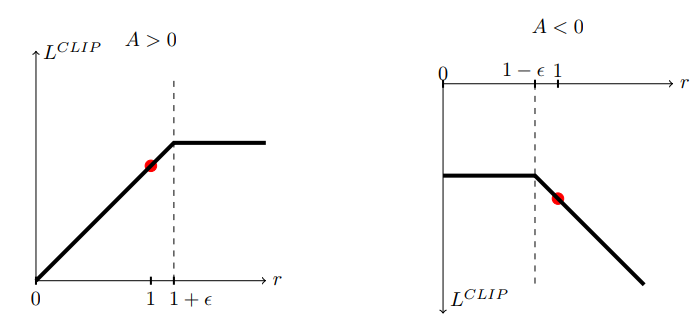
\includegraphics[width=80mm,scale=1]{PPO Clip.png}
    
    \caption{Clip Function Limiting the Size of the Step Taken \cite{DBLP:journals/corr/SchulmanWDRK17}}
    \label{fig:my_label}
\end{figure}

\subsection{PPO in Rocket League}
 In complex and high-dimensional environments like Rocket League, PPO can be used to train an agent to 
 effectively navigate the action space and make decisions based on a large number of observation inputs.

 For example, in Rocket League, the action space consists of a wide range of inputs that the agent can 
 take. These inputs include, but are not limited to: boosting, air-rolling, moving in any direction, 
 accelerating, decelerating, powersliding (drifting), jumping, and any combination of these actions.

 Additionally, the agent has access to a variety of observation inputs, including the location of the 
 ball, the amount of boost available, the location of teammates and opponents, the velocity of the ball 
 and other cars, the distance to the ball and other cars, the angle of the car relative to the ball and 
 other cars, the orientation of the ball, the state of the game (e.g. whether it is a kickoff, in play, or 
 a goal has been scored) the score of the game and the remaining time. These observation inputs can 
 provide valuable information for the agent to make decisions and take actions in the game. Overall, the 
 combination of the high-dimensional action space and the rich set of observation inputs makes Rocket 
 League a challenging but rewarding environment for training reinforcement learning agents.

 One of the key advantages of PPO is that it is relatively simple to tune the algorithm's parameters, 
 which makes it scalable to larger models. This is important in environments like Rocket League, where the 
 action space is high-dimensional and the game is computationally complex. Additionally, PPO is designed 
 to minimize the cost function at each step while ensuring that the new policy does not deviate too much 
 from the previous policy. This provides confidence that the policy update will not take a step that is 
 too large and fall off of the "gradient cliff," resulting in random, unintended behaviors. By choosing 
 appropriate step sizes, PPO can be effective in continuous environments like Rocket League.

 Overall, PPO is a promising approach for training reinforcement learning agents in complex and high-
 dimensional environments like Rocket League. By simplifying the policy gradient methods and carefully 
 controlling the policy updates, PPO can help to mitigate some of the challenges that are commonly 
 encountered in DRL algorithms; hence, this is the algorithm used to train the agent to learn the game 
 Rocket League.

\section{Prior Work}
 The use of reinforcement learning in video games is not a novel idea. A machine called "AlphaGo" was 
 trained via reinforcement learning to play the game Go. In terms of complexity, Go is "profoundly 
 complex" with more possible game configurations than there are known atoms in the universe 
 \cite{deepmind}. \textcite{deepmind} states that prior to their machine, AI was only able to play at the 
 amateur level. After thousands of games of playing against itself, through reinforcement learning, AlphaGo
 was able to sweep a professional Go player 5-0 in 2015. Later, it was able to beat the world's best Go 
 player. OpenAI Five is another machine that was trained via reinforcement learning to play the game Dota 
 2\cite{OpenAI_dota}. Dota 2 is a 5v5 battle-arena video game, that involves teamwork in order to achieve 
 victory. OpenAI Five was trained for 180 years per day on 256 GPUs and 128,000 CPU cores. In 2019, OpenAI 
 Five swept a world champion Dota 2 team 2-0. This agent was trained on a complex Deep Reinforcement 
 Learning model that incorporated a long short term memory neural network in it.

 
\subsection{RLBot}
 For the game of Rocket League, Psyonix had developed four levels of AI: "Beginner," "Rookie," "Pro," and 
 "All-Star." The highest level of bot, All-Star, is equivalent to the rank of silver in Rocket League, 
 which is the second lowest rank in the game. This was unfortunate because, as players got better than 
 these bots, there really were no challenges or opportunities to practice in low-stakes environments to 
 further improve. This inspired the RLBot framework to be developed. RLBot enabled programmers to hard- 
 code their own bots using an understanding of the physics and mathematical principles of the game. This 
 allowed for the creation of much better bots; however, these bots could reach nowhere near any of the top 
 competitive ranks.

\subsection{RLGym}
 Then came along the Python API called RLGym. Using a Rocket League mod called BakkesMod, RLGym was able to turn Rocket League into an OpenAI gym environment. This allowed for users to train bots via reinforcement and deep reinforcement learning. Due to the high dimensionality and infinite action space full of rich, spatio-temporal data, AI developers are optimistic about utilizing RLGym for machine learning within the game of Rocket League \cite{inproceedings}.

\subsection{Nexto: The Best Rocket League Bot}
 Currently, the best Rocket League "community bot" is called Nexto. It is trained via deep reinforcement 
 learning using the computational power of many people within the Rocket League community. This bot's 
 predecessor, "Necto," was determined to be around the high diamond rank \cite{github}. The team took what 
 they learned from Necto and started fresh in training Nexto. This resulted in Nexto reaching what is 
 considered low grand champ 1 rank, which is 2 ranks above Necto. While it is currently not explicit how 
 long Nexto has trained, there is a gif on the Necto Github repo that says Necto (at one point) had been 
 trained for 9 years, 9 weeks, and 3 days. Necto also won the 2022 RLBot championship by a considerable 
 margin each game.

\section{Methods}

\subsection{Tuning Hyperparameters}
In the early stages of training, the learning rate and batch 
size were tuned to be higher in order to allow the agent to 
quickly explore the environment and learn as much as 
possible. This allowed the agent to discover different 
strategies and tactics that it could use to succeed in the 
game of Rocket League.

As the agent continued to train, the learning rate and batch 
size were gradually adjusted to be lower in order to allow 
the agent to more carefully exploit what it had learned in 
the early stages of training. This helped the agent to focus 
on using its existing knowledge to make more accurate 
predictions and decisions, rather than continuing to explore 
the environment in a haphazard manner.

In addition, the number of training steps and epochs were 
carefully chosen to ensure that the agent had enough time to 
explore and learn in the early stages of training, while also 
limiting the amount of time it spent on exploration in the 
later stages of training. This allowed the agent to strike a 
balance between exploration and exploitation, allowing it to 
learn as much as possible in the early stages of training 
while also using its existing knowledge to make accurate 
predictions and decisions in the later stages of the game.

 \subsection{Current Rewards}
 In the Oswald reward, the rewards are determined based on events that occur in a game of Rocket League. These events include scoring goals, conceding goals, touching the ball, taking shots, making saves, and picking up boost. The weights for these events can be adjusted to fine-tune the reward function for a specific learning task. The reward is calculated based on the accumulation of events over the course of the game, rather than the events that occur in a single episode. This allows the reward function to provide a more comprehensive assessment of the agent's performance. The subsequent rewards are the aforementioned ball-oriented rewards.

 The player to ball reward is based on the distance, direction, and speed of the player and ball. The reward is adjusted based on these factors, with the distance and speed being the most important. If the player is moving towards the ball, the reward is increased, and if the player is moving away from the ball, the reward is decreased. The hit speed reward is an incentive for hitting the ball cleanly and powerfully. The airdribble reward function is similar to the player to ball reward; however, it additionally rewards the agent for keeping the ball close to it while both the agent and the ball are in the air. This is an incentive for eliciting the airdribble mechanic. This reward is weighted lower than the others to prevent from unintended behaviors because airdribbling is more of a difficult/advanced mechanic. The ball to goal reward calculates the distance between the ball and the goal and returns a reward if the ball is moving towards the goal; otherwise, the agent is given a tiny punishment. Finally, the agent is encouraged to be moving via a small fraction of the agent's linear velocity as a reward.

\subsection{Normalization of the Rewards}
 The rewards that were passed to the agent were normalized.  This is an important step because it helps to ensure that the agent does not become overly fixated on a single reward and instead rewards and punishes when appropriate. Normalizing rewards is a process that involves scaling the reward values so that they are in the same range and can be used to measure the effectiveness of the agent’s policy \cite{weng_2020}. This helps the agent to recognize trends in the reward values, which it can use to further improve its policy.

\subsection{Custom Observations}
 The observations passed to the agent include information about the current state of the game, such as the positions and velocities of the ball and the players, as well as information about the previous action taken by the agent. This allows the agent to have a complete view of the game and allows the agent to learn policies that maximize the reward. The observations are also normalized to ensure that they have consistent ranges, which can improve the performance of the agent \cite{brummerloh_2021}. Other observations include: boost amount, whether the agent is on the ground, whether the agent has a flip, whether or not the agent is demolished, the orientation of the agent in relation to the game world, and information about its relative position to the goal it is attacking and the goal it is defending.

\subsection{Neural Network Architecture and Actor-Critic Model}
 The net architecture of this actor-critic PPO model includes 
 three fully connected layers for the policy network, each 
 with 512 units, and three fully connected layers for the 
 value network, each with 400 units. The use of fully 
 connected layers allows the model to learn a complex 
 function that can map the input observations to actions and 
 values.

 Having a larger actor network than critic network is 
 beneficial because the actor is responsible for selecting 
 actions in the environment, which can have a larger impact 
 on the overall performance of the model. A larger and more 
 complex actor network allows the model to learn more 
 sophisticated policies that can improve its ability to 
 succeed in learning how to play the game \cite{neal2019in}.

\subsection{Custom State Setters}
 Custom state setters were created in order to have the agent start learning from a variety of different initial conditions, rather than always starting from the same state. The custom states created were fashioned in such a way as to create a curriculum training scheme for the agent. One of the main advantages is that it can speed up the learning process by allowing the agent to learn simple skills quickly and move on to more complex tasks. This can reduce the amount of training time required and make it easier for the agent to learn to solve a wide range of tasks \cite{https://doi.org/10.48550/arxiv.2003.04960}.
 
 The first task focused on offensive play, with the reset method setting the initial state of the game such that the ball is placed in front of the opponent's goal. This would allow the agent to learn how to score goals by shooting or redirecting the ball into the goal. The task focused on defensive play, with the ball placed in front of the agent's own goal. This would allow the agent to learn how to save the ball by blocking shots. Finally, the task was geared towards dribbling and ball control. The ball was placed on top of the agent's car. This would allow the agent to learn how to dribble and flick the ball to maintain possession and set up scoring opportunities.

\subsection{Training the Agent}
 The main routine of training the agent involved roughly three days of continuous training, and then the agent's behaviors would be observed in order to assess its progress. Based on the analysis of the behaviors, the rewards, observations, and hyperparameters would be adjusted in order to try and elicit better behaviors from the agent and improve its overall performance. This process of observing, analyzing, and adjusting would continue throughout the training process in order to gradually improve the agent's performance.
 
\section{Evaluation}

\subsection{Model Metrics}
 Tensorboard was used to analyze how the neural network was 
 performing, and to gauge whether or not the model was 
 minimizing the loss while maximizing the reward. These 
 metrics were assessed in light of how the agent actually 
 performed in matches and the observed behaviors when put 
 into a low stakes environment. All of the Tensorboard data 
 is not included in the paper; however, it can be found under 
 the "logs" directory in the Github, which can be uploaded to 
 Tensorboard in order to view all of the training graphs.

\subsection{Intelligence, Wins and Losses, Point Breakdown}

 Evaluation would occur both qualitatively and 
 quantitatively. Game play in 1v1 matches would be observed 
 for intelligent behaviors. This could be chasing after the 
 ball, hitting the ball, rotating from offense to defense and 
 vice versa, etc. The bot would also be judged off of whether 
 or not it won or lost the game. Models will also be trained 
 against other models that were trained that have different 
 neural architectures, reward functions, and other potential 
 differences that might help converge upon training settings 
 that would help produce the best bot possible. Finally, 
 pending the results of the training and findings, the bot 
 could be tested against low-skilled human players as well. 

\section{Results and Discussion}

\subsection{Custom Reward Shaping: A Blessing and a Curse}

 As previously described, the curse of dimensionality is a significant challenge in the development of 
 reinforcement learning algorithms. As the number of dimensions in the state space increases, the number 
 of possible combinations of states and actions also increases exponentially, which can make it difficult 
 for the learning algorithm to effectively learn the optimal behavior. In the context of Rocket League, 
 this can lead to issues with reward hacking and the need to carefully design the reward function to 
 provide guidance to the learning algorithm. Custom rewards, built using domain knowledge, can be used to 
 reduce the dimensionality of the action space and improve training efficiency and generalization.
 
 However, it became apparent that custom rewards built using 
 knowledge of the domain can actually end up 
 hindering/lengthening the training process if not done 
 methodically. Creating too many rewards and punishments resulted in non-optimal or even counter- productive behavior, as was observed in the evaluation of the 
 agent's behaviors. When put into a real game scenario, the agents demonstrated a way in which they exploited the reward for facing the ball by simply sitting 
 still and facing the ball, rather than attempting to face the ball and drive into it. When manually bumped, the agent began to move and 
 exploited another reward for touching the ball in the air, 
 leading them to repeatedly drive backwards up the ceiling 
 and then falling off the ceiling in an attempt to hit the 
 stationary ball. This behavior not only hindered the agents' 
 ability to score goals, but also increased the training time 
 required to teach the agents more effective strategies.
 
 To combat this, a velocity reward was added to encourage the 
 agents to move quickly. However, the agents exploited this 
 reward by performing a well-known mechanic in the game 
 called a "speed-flip," which allowed them to quickly 
 accelerate to their maximum speed by diagonally flipping. 
 While this was impressive to see, the agents still did not 
 attempt to score goals or interact with the ball.
 
 These observations led to the creation of, the current, 
 strictly ball-oriented rewards, in addition to the existing 
 rewards for in-game events such as scoring and getting 
 scored on. By carefully designing the rewards to 
 specifically encourage the desired behavior, the training 
 process was able to progress more efficiently and 
 effectively — as the agent began touching the ball more 
 often and earlier in its training.

\subsection{The Current Agent: Optimizing the Reward}

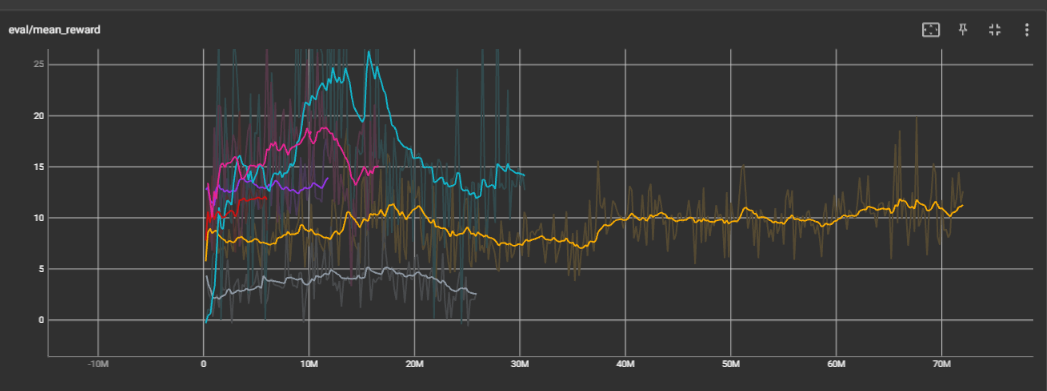
\includegraphics[width=3in,scale=1]{reward_graph.png}

 Paired with the visual observations of the agent touching 
 the ball more often in a low-stakes environment outside of 
 its training environment, the graph of the mean reward is 
 able to verify that these behaviors are not happening solely 
 by chance. The mean reward of the agent trained with the 
 ball-oriented rewards is indicated by the cyan color line. 
 The other colored lines are previous iterations with over- 
 saturated rewards/punishments along with other 
 hyperparameters that happened during the training process. 
 This graph is generated by taking the mean value of the 
 reward from the last 30 episodes. Visually, it can be seen 
 that the agent starts off with a random policy (indicated by 
 almost 0 mean reward value) and then quickly begins 
 optimizing the reward in the first twenty million timesteps. 
 Due to the fact that almost every single reward involves the 
 ball being touched, paired with the visual behavioral 
 confirmation of the agent touching the ball more during 
 training, confirms that the agent is beginning to learn that 
 the ball plays a crucial role in "solving" how the game is 
 played. These results are quite encouraging and provide 
 confidence that something the rewards are being exploited 
 and the agent is headed down the right path for learning how 
 to play the game of Rocket League.


 \subsection{Training and Time Consumption}
 Even though the agent is beginning to touch the ball more 
 often and less randomly, it is still not ready to be 
 evaluated in an actual game. The over-saturation of rewards 
 and punishments set the project back quite a bit. The shift 
 towards all ball-oriented rewards had taken place after 
 three weeks of training on a single model. Time then had to 
 be taken to write new, ball-oriented rewards and tune the 
 observations accordingly. Even with the new model, 
 hyperparameters were constantly being adjusted in order to 
 attempt to achieve the desired results; however, these 
 changes sometimes led to unexpected outcomes that required 
 additional time to address.
 
 Another factor that contributed to the time-consuming nature 
 of training the agent was the use of multiple instances of 
 the game. In order to train the agent effectively, it was 
 necessary to run the game on multiple instances 
 simultaneously, often overnight, in order to gather 
 sufficient data. However, this approach was not without its 
 challenges, as the game would often crash, requiring the 
 training to be restarted which could not always be done 
 immediately.
 
 Ultimately, the complexity of the game, combined with the 
 need to start models from scratch, constantly adjust rewards 
 and hyperparameters, and the challenges of running multiple 
 instances of the game for extended periods of time, made 
 training a reinforcement learning agent to play Rocket 
 League a time-consuming endeavor. As a result, it was not 
 possible to produce a model that played the game well in the 
 amount of time originally allotted for training.


\subsection{The Future of Oswald}
 Given the promises of the current iteration of training with 
 strictly ball-oriented rewards, Oswald will continue 
 training so that it can get to the point of formal match 
 evaluations. Upon reading discourse from the RLGym Discord 
 server, it appears that most agents have aspects of the game 
 hard-coded so that they are executed perfectly every time. 
 The main situation in which this is done is for kick-offs. 
 Winning a kickoff to immediately go into the opponent's half 
 provides a huge advantage, especially in 1v1 games. This 
 will be implemented into Oswald's observations and actions. 
 
 Ultimately, the thing Oswald need's the most right now is 
 time. Time to train and sharpen its heuristics so that it 
 can become the ultimate scoring machine. As the designer, 
 not being able to formally evaluate the agent outside of its 
 behaviors is extremely unsatisfactory. Hence, Oswald will 
 continue to train for the following months, rewards and 
 hyperparameters will be tweaked accordingly, and match 
 evaluations will take place in the future. 


\section{Ethical Considerations}
 Implementing deep reinforcement learning within the video 
 game Rocket League does not need to account for too many 
 ethical considerations; however, the use of such algorithms 
 within the real world does. Problems that arise from DRL 
 machines within complex video game environments can actually 
 help foreshadow some of the issues that might arise in a 
 larger scale setting. Ultimately, it is imperative that we 
 take time to make ethical considerations about how such 
 technology might affect society and what precautions may be taken in order to mitigate the possible detriments.

 As researches make advances in Artificial Intelligence, 
 governments, organizations, and the general public seek to 
 understand and implement this technology into everyday life 
 \cite{SchiffBBL20}. Deep Reinforcement Learning has greatly 
 contributed to the pervasive hype around AI and its 
 possibilities. With the rapid growth in popularity and 
 progress, it is important to consider the societal and 
 ethical implications that such technology imposes for the 
 future. Studies have already shown how the implementation of 
 AI has resulted in racism/discrimination, algorithmic bias, 
 technological unemployment, and many other challenges that 
 researchers must circumvent in hopes of creating an 
 equitable and ethical future \cite{SchiffBBL20}.

\subsection{DRL in Competitive Rocket League}
 Ethical concerns begin to rise as DRL Rocket League bots 
 become better trained. Rocket League is a competitive Esport 
 that has large cash prizes for many of the major 
 tournaments. Outside of the professional scene, there is 
 also a ranked game mode in which many people grind to 
 achieve the highest rank of Supersonic Legend and make their 
 way onto the top leader boards. When these DRL agents 
 surpass the abilities of human Rocket League players, they 
 may find themselves being abused in ranked matches and 
 perhaps could be used to help boost players to higher ranks 
 that they do not actually deserve. In this regard, if these 
 agents were able to enter the competitive scene without 
 others being explicitly aware of their presence, it would 
 ruin the integrity of the game; and, negate the dedication 
 of players who are trying to make the ranked climb 
 earnestly. In an extreme case, someone might figure out a 
 way to have agent play for them in the Esports scene to help 
 them win major tournaments. Again, this would ruin the 
 integrity of the game, and the individual using the unfair 
 agent would essentially be stealing money from the 
 tournaments.

\subsection{Data Collection Issues}

 Outside of Rocket League, the methods of trial-and-error 
 used in DRL to learn optimal policies cannot be used in high 
 stakes, real-life settings. Collecting data to find the 
 optimal policies for creating cogent texts through NLPs, 
 making clinical decisions, making money in the stock market, 
 or creating self-driving cars would require performing trial-and-error experiments at the potential cost of being 
 offensive, losing money, and even at the cost of human 
 lives. A machine cannot blow through a stoplight and cause a 
 deadly car accident, make an awful trade that loses a large 
 part of one's portfolio, generate profusely offensive text, 
 or prescribe a treatment to someone that ends up killing 
 them before the machine learns to stray away from such bad 
 behaviors \cite{10.1613/jair.1.12360}. Simulations may 
 provide environments for training; however, they may not be 
 complex enough to learn and account for every nuance of 
 everyday life. Data collection may also be expensive to 
 obtain, or may infringe on people's privacy. Thus, some 
 parameters may be overlooked or excluded by the machine — 
 leading to more unintentional consequences or discrimination.

\subsection{Reward Hacking}
 In the same vein exists the issue of reward hacking by the 
 machine. Much like humans, machines will exploit shortcuts 
 to maximize gain when they are available. If a DRL machine 
 explores and finds a policy that maximizes a reward, it will 
 perform those actions of the policy regardless of whether or 
 not it actually achieves the intended goal. In a real world, 
 high stakes setting, there is no room for error. Especially 
 as objectives become more nuanced and pose high-dimensional 
 problems, reward shaping becomes exponentially more complex; 
 and, there exist more opportunities for the machine to find 
 ways to exploit rewards via a means that do not achieve the 
 desired goal \cite{frye_2021}.

\subsection{Energy Consumption}
 For this project, multiple instances of Rocket League were 
 run on a single computer for extended periods of time, which 
 has ethical implications related to energy consumption, 
 particularly when it comes to training large and complex 
 models. As the size and complexity of the model increase, 
 the amount of computational power needed to train the model 
 also increases. This, in turn, requires more energy to run 
 the computer and keep it cool.

 Furthermore, the use of large and complex models in 
 reinforcement learning research often requires running 
 multiple instances of the game simultaneously, which can 
 further increase the energy consumption. This is because 
 large and complex models often require a large amount of 
 data to train effectively, and running multiple instances of 
 the game can generate more data more quickly.

 The use of large-scale language models in natural language 
 processing (NLP) research has garnered significant attention 
 in recent years, with models such as GPT-3 and the Switch 
 Transformer achieving impressive performance on a range of 
 tasks. However, the environmental impact of training and 
 serving these models has also been a topic of concern, with 
 some research estimating that the carbon emissions from 
 training a single large-scale model can be equivalent to the 
 lifetime emissions of multiple cars \cite{gupta_2021}.
 
\printbibliography
\end{document}